\chapter{Dimensionality reduction, indexing and bounding.}
As we seen with application of LCS to images in \cite{citeulike:4367061} Yazdani and Ozsoyoglu charachterized each of the images by the set of Fourier coefficients. By employing such a solution they managed to resolve the ``dimensionality curse'' in the time series-similarity problem which essentially decreases the performance of any similarity algorithm to the one of the sequential search with the growth of dimensionality above 16 cite{citeulike:4408223} \cite{citeulike:4384496} \cite{citeulike:2843857} \cite{citeulike:4384489} \cite{citeulike:343069}.

The problem addressed in this chapter is the approximation (lossy compression) of a time series data in a way which allows to maintain a fast random access, comparison and indexing of the time-series with minimal errors. There are many approximation proposed in the research literature and the Figure \ref{fig:approximations} from \cite{citeulike:2821475} illustrates their hierarchy. All of the methods essentially at the first step transform given set of time series into some low-dimensional representation and index them in order to utilize data-mining, indexing and clustering algorithms later. Key questions we would ask in this review of the reduction methods are the sensitivity and selectivity of algorithms, their complexity and performance.

\begin{figure}[tbp]
   \centering
   \includegraphics[height=45mm]{ts_representations.eps}
   %%{seriesheatmap}
   \caption{The figure from \cite{citeulike:2821475} illustrating a hierarchy of all of the flavors of time series representation (decomposition).}
   \label{fig:approximations}
\end{figure} 
